\author{Philipp Dominik Bzdok}

\title{Bachelorarbeit Medientechnologie \linebreak \linebreak
Authentifizierungsmethoden für digitale Fernsignaturen auf Grundlage der Handy-Signatur}

\documentclass[11pt,a4paper,ngerman]{report}
\usepackage[T1]{fontenc}
\usepackage{fontspec}
\usepackage[ngerman]{babel}

\usepackage{fancyhdr}
\pagestyle{fancy}
\fancyhf{}
\setlength{\headheight}{14pt}
\fancyhead[R]{\textsl{\rightmark}}
\fancyfoot[R]{\thepage}

\fancypagestyle{plain}{%
    \renewcommand{\headrulewidth}{0pt}%
    \fancyhf{}%
    \fancyfoot[R]{\thepage}%
}

\usepackage{color}
\usepackage{tabularx}
\usepackage{amsmath}
\usepackage{amssymb}
\usepackage{graphicx}
\usepackage[skip=5pt,font=footnotesize]{caption}

\usepackage{todonotes}

\usepackage[titles]{tocloft}
\newlistof{listing}{lol}{Quellcodeverzeichnis}

\usepackage[newfloat]{minted}
\usemintedstyle{xcode}
\setminted[java]{linenos,tabsize=2,breaklines,fontsize=\footnotesize,frame=lines,framesep=2ex,autogobble}
\setminted[ruby]{linenos,tabsize=1,breaklines,fontsize=\footnotesize,frame=lines,framesep=2ex,autogobble}

\usepackage{hyperref}
\hypersetup{pdfborder={0 0 0}, breaklinks=true}

\setlength{\parskip}{0.5em}
\setlength{\parindent}{0em}

\setlength{\cftlistingnumwidth}{3em}

\newcommand{\ruby}[1]{\mintinline{ruby}{#1}}

% !TEX root = Bachelorarbeit_Philipp_Bzdok

\begin{document}
\maketitle

% ----------------------------------------------------------------
% Preamble DE
% ---------------------------------------------------------------- 
\chapter*{Bachelorarbeit}
\textbf{Thema:}

Authentifizierungsverfahren für digitale Fernsignaturen auf Grundlage der Handy-Signatur
\\[4ex]
\textbf{Gutachter:}
\begin{enumerate}
    \item Prof. Dr.-Ing. Luigi Lo Iacono (Technische Hochschule Köln)
    \item Dipl.-Ing. Tobias Wagner (n-design GmbH)
\end{enumerate}
\textbf{Zusammenfassung:}

Die digitale Signatur stellt ein wichtiges Werkzeug der modernen Informationstechnik dar und durch Fernsignaturen ist es heutzutage möglich, digital, rechtsgültige Unterschriften zu leisten. Der Prozess der Signatur setzt dementsprechend eine starke Authentifizierung des Benutzers voraus. In diesem Kontext wird die SMS-TAN, das erste Authentifizierungsverfahren der österreichischen Handy-Signatur und das am weitesten verbreitete Zwei-Faktor Authentifizierungsverfahren, analysiert. Darauf aufbauend werden alternative Authentifizierungsverfahren für den Anwendungsbereich Fernsignatur evaluiert. Durch die prototypische Implementierung der TOTP und U2F Authentifizierungsverfahren wird gezeigt, wie mit überschaubarem Aufwand die unsichere SMS-TAN substituiert werden kann um somit ein höheres Sicherheitsniveau zu erreichen.
\\[4ex]
\textbf{Stichwörter:}

Authentifizierung, digitale Signatur, Kryptographieverfahren, SMS-TAN, TOTP, U2F
\\[4ex]
\textbf{Datum:}

\today
\clearpage

% ----------------------------------------------------------------
% Preamble EN
% ---------------------------------------------------------------- 
\chapter*{Bachelors Thesis}
\textbf{Title:}

Authentication procedures for digital remote signatures based on mobile phone signatures
\\[4ex]
\textbf{Reviewers:}
\begin{enumerate}
    \item Prof. Dr.-Ing. Luigi Lo Iacono (Technische Hochschule Köln)
    \item Dipl.-Ing. Tobias Wagner (n-design GmbH)
\end{enumerate}
\textbf{Abstract:}

The digital signature is an important tool of modern information technology and with remote signatures it is now possible to provide digital, legally valid signatures. Accordingly, the signature process requires a strong authentication of the user. In this context, the SMS-TAN, the first authentication procedure of the Austrian mobile phone signature and the most widespread two-factor authentication procedure, is analyzed. Based on this, alternative authentication methods for the field of remote signatures will be evaluated. Through the prototypical implementation of the TOTP and U2F authentication methods, it will be shown how the unsecure SMS-TAN can be substituted with a manageable effort in order to achieve a higher level of security.
\\[4ex]
\textbf{Keywords:}

Authentication, digital signature, cryptographic methods, SMS-TAN, TOTP, U2F
\\[4ex]
\textbf{Date:}

\today
\clearpage

% ----------------------------------------------------------------
% Eidesstattliche Erklärung
% ---------------------------------------------------------------- 
\chapter*{Eidesstattliche Erklärung}
Ich erkläre an Eides statt, dass ich die vorgelegte Abschlussarbeit selbständig und ohne fremde Hilfe verfasst, andere als die angegebenen Quellen und Hilfsmittel nicht benutzt und die den benutzten Quellen wörtlich oder inhaltlich entnommenen Stellen als solche kenntlich gemacht habe.

\vspace{1.5cm}

\_\_\_\_\_\_\_\_\_\_\_\_\_\_\_\_\_\_\_\_\_\_ \\
(Ort, Datum)

\vspace{0.5cm}

\_\_\_\_\_\_\_\_\_\_\_\_\_\_\_\_\_\_\_\_\_\_ \\
(Unterschrift)

\clearpage

% ----------------------------------------------------------------
% Vorwort
% ---------------------------------------------------------------- 
\chapter*{Vorwort}
Hier möchte ich auf die Umstände der Abschlussarbeit eingehen und denen danken, die mir dabei geholfen haben.
\clearpage

% ----------------------------------------------------------------
% Inhaltsverzeichnis
% ---------------------------------------------------------------- 
\tableofcontents
\clearpage

% ----------------------------------------------------------------
% Inhalt
% ----------------------------------------------------------------

\chapter{Einleitung}
Digitale Signaturen nehmen in der heutigen Zeit eine wichtige Rolle in der Informationstechnik und somit im Alltag ein. Mit Hilfe von digitalen Signaturen ist es möglich beliebigen Daten zweifelsfrei Integrität und Authentizität nachzuweisen. Die Eigenschaften der Integrität und Authentizität sind besonders wichtig im juristischen Kontext der elektronischen Signatur, in welchem sie das Gegenstück zur handschriftlichen Unterschrift bildet. Der Begriff elektronische Signatur wird oft synonym zur digitalen Signatur verwendet, jedoch ist die elektronische Signatur ein juristischer Begriff, welcher erstmals in einem überarbeiteten Entwurf der EU-Richtlinie 1999/93/EG von der EU-Kommission verwendet wurde \cite{eSigEU99}. Der Begriff digitale Signatur hingegen stammt aus der Mathematik beziehungsweise aus der Kryptographie und bezeichnet einerseits ein asymmetrisches Kryptographieverfahren, aber anderseits den mathematischen Wert welcher durch das Kryptographieverfahren erzeugt wird.

Digitale Signaturen werden bereits in einem breiten Spektrum von Anwendungen eingesetzt, wie zum Beispiel in PGP-Systemen\footnote{Pretty good Privacy - 1986 bis 1991 von Phil Zimmermann entwickelt.} oder Zertifikatsbasierten Systemen. Des weiteren werden digitale Signaturen immer häufiger in neuen Anwendungsbereichen eingesetzt. Eine besondere Anwendung auf die ich im Laufe dieser Ausarbeitung explizit eingehen möchte, ist die österreichische \textit{Handy-Signatur}. Die \textit{Handy-Signatur} ermöglicht es den Bürgern Österreichs sich ohne zusätzliche Hardware, wie Kartenlesegeräte, online per Handy auszuweisen oder Formulare und Dokumente elektronisch zu unterschreiben \cite{handySigOnline}. Die Besonderheit dieser digitalen Signatur ist, dass die \textit{Handy-Signatur} eine qualifizierte elektronische Signatur auslöst und somit juristisch einer handgeschriebenen Unterschrift gleichgesetzt werden kann. Die für die Signatur benutzte Authentifizierungsmethode ist die mobile \textit{SMS-TAN}. Diese Authentifizierungsmethode wurde jedoch bereits von \textit{NIST}\footnote{National Institute of Standards and Technology} in ihrer Tauglichkeit eingeschränkt, da SMS nie dafür gemacht worden ist Geheimnisse zu übertragen \cite{mobileSec,NIST800-63B}. Trotz der mangelhaften Eignung von SMS als Kanal für OOB-Authentifizierung\footnote{Out-Of-Band Authentifizierung - Authentifizierung über separaten Kanal}, ist das SMS-OTP\footnote{One time password} die am meisten verbreitete Variante der multifaktor Authentifizierung \cite[Abb. 3]{fido17}.

Aus diesem Grund möchte ich in dieser Arbeit die Eigenschaften der Authentifizierungsmethode der \textit{Handy-Signatur} beleuchten und darauf basierend Alternativen evaluieren und prototypisch implementieren. Mein Ziel ist es, die modernen Möglichkeiten von Multi-Faktor Authentifizierung im Kontext der digitalen Signatur zu vergleichen und zu bewerten, um abschließend eine Aussage über die Tauglichkeit für den Anwendungsbereich \textit{Fernsignatur} machen zu können.

\section*{Abgrenzung}
Die digitale (Fern-)Signatur besteht aus vielen komplexen Verfahren, wie Hash-Funktionen, digitale Signaturen, Smartcards, uvm.. Diese möchte ich nur der Vollständigkeit halber erläutern. In diesen Bereichen werde ich mich nur auf bereits veröffentlichte Methodiken stützen und von ihnen gebrauch machen.
\clearpage


\chapter{Grundlagen}
Um die Eignung von Authentifizierungsmethoden bestimmen zu können, müssen erst einmal die Rahmenbedingung festgelegt werden. Die digitale Signatur und die \textit{Handy-Signatur} werden im folgenden beleuchtet, da dies der Anwendungsbereich ist, welchen die Authentifizierungsmethoden schützen sollen. Dazu stelle ich verschiedenste Signaturvarianten und deren Komponenten im Detail dar. Nach der Bestimmung dieser Eigenschaften wird die Authentifizierung im Kontext der Signatur erläutert.

\section{Hash-Funktionen}\label{sec:Hash-Funktionen}
\textit{Hash-Funktionen} spielen eine zentrale Rolle in der Welt der Kryptographie und \textit{digitalen Signaturen}. Allgemein bilden diese Funktionen eine Nachricht beliebiger (Bit-)Länge auf einen Hash-Wert festen Länge ab. Der Hash-Wert ist abhängig von der gesamten Nachricht und sollte möglichst schnell berechnet werden können. Eine weitere besondere Eigenschaft von kryptographischen \textit{Hash-Funktionen} ist die Kollisionsfreiheit, wie in \cite[S. 89]{krypt08} beschrieben: 
\begin{quote}
    ``Es sei $M$ eine Nachricht. Eine Hashfunktion $h$ ist \textit{schwach kollisionsfrei für $M$} [...], wenn es berechnungsmäßig praktisch unmöglich ist, eine Nachricht $M' \neq M$ mit $h(M) = h(M')$ zu finden. [...]
    Eine Hashfunktion ist \textit{stark kollisionsfrei} [...], wenn es berechnungsmäßig praktisch unmöglich ist, Nachrichten $M$ und $M'$ mit $M' \neq M$ und $h(M') = h(M)$ zu finden.''
\end{quote}
Für die Verwendung von \textit{Hash-Funktionen} im Kontext der Signatur muss die Funktion eine sogenannte \textit{Einweg-Hash-Funktion} sein, wie in \cite[S. 99]{krypt08} beschrieben:
\begin{quote}
    ``Eine Hashfunktion ist eine \textit{Ein-Weg-Funktion} [...], wenn es für einen gegebenen Fingerabdruck $z$ berechnungsmäßig praktisch unmöglich ist, eine Nachricht $M$ mit $h(M)=z$ zu finden.''
\end{quote}
Implizit ergibt sich aus der Forderung nach stark kollisionsfreien \textit{Hash-Funktionen} auch die Eigenschaften der Ein-Weg-Funktionen \cite[S. 99]{krypt08}.

Die \textit{Hash-Funktionen} sind so wichtig für die \textit{digitalen Signaturen}, da bei den gängigen Signaturvarianten nur der Hash-Wert der Nachricht signiert wird und nicht die Nachricht selbst. Wichtige Funktionen in diesem Kontext, die in ihrer Sicherheit stetig durch führende Institutionen (NIST\footnote{National Institute of Standards and Technology - Secure Hash Standard \cite{shs180-4}}, BSI\footnote{Bundesamt für Sicherheit in der Informationstechnik \cite[Kapitel 4]{bsi-tr-02102-1}}, etc.) geprüft werden, sind:
\begin{table}[h]
    \begin{tabularx}{\textwidth}{ |X|X| }
        \hline
        SHA2 & SHA-256, SHA-512/256, SHA-384 und SHA-512 \\
        \hline
        SHA3 & SHA3-256, SHA3-384, SHA3-512 \\
        \hline
    \end{tabularx}
    \caption{Empfohlene Hash-Funktionen}
    \label{table:Hashfunktionen}
\end{table}

Eine Signatur soll die Eigenschaften Integrität und Authentizität haben. Damit die Authentizität gewährleistet werden kann, muss erst die Integrität der Nachricht sicher gestellt werden. An dieser Stelle greifen die Eigenschaften der \textit{Hash-Funktion}. Dadurch, dass nur der Hash-Wert signiert wird, kann der Empfänger der Signatur durch eine eigene Hash-Wert Berechnung der Nachricht sicherstellen, dass die Nachricht nicht verändert worden ist. Außerdem bietet die Signatur des Hash-Wertes mit fixer Länge Laufzeitvorteile in einigen Signaturverfahren.

\section{Digitale Signaturen}
Als \textit{digitale Signatur} bezeichnet man im allgemeinen ein asymmetrisches Kryptosystem\footnote{Oberbegriff für Public-Key-Verschlüsselungsverfahren}. Bei asymmetrischen Kryptographiesystemen besitzt jeder Teilnehmer ein Schlüsselpaar, bestehend aus einem \textit{öffentlichen Schlüssel} und einem \textit{privaten Schüssel}. Der \textit{private Schlüssel} wird für den Signaturalgorithmus verwendet, wobei der \textit{öffentliche Schlüssel} von einer beliebigen anderen Person abgerufen werden kann um die Signatur zu verifizieren (siehe Abb. \ref{fig:Signaturablauf}). Da ausschließlich der Teilnehmer selbst Zugang zu seinem eigenen \textit{privaten Schlüssel} hat, eignet sich ein solches System hervorragend zur Sicherstellung von Authentizität von Daten und somit zur \textit{digitalen Signatur}. Authentizität ist eine der fünf wichtigen Eigenschaften einer Signatur \cite{sch05}:
\begin{enumerate}
    \item Sie ist \textbf{authentisch}. Das bedeutet, dass der Unterzeichner die Signatur willentlich ausgeführt hat.
    \item Sie ist \textbf{fälschungssicher}. Das bedeutet, dass die Signatur ausschließlich vom Unterzeichner ausgeführt worden ist und von niemand anderen.
    \item Sie ist \textbf{nicht wiederverwertbar}. Das bedeutet, dass die Signatur nur auf einer Nachricht gültig ist.
    \item Die signierte Nachricht ist \textbf{unveränderbar}. Das bedeutet, dass die Nachricht nach der Signatur nicht modifiziert werden kann.
    \item Die Signatur ist \textbf{bindend}. Das bedeutet, das der Unterzeichner diese zu einem späteren Zeitpunkt nicht annullieren oder bestreiten kann.
\end{enumerate}
\begin{figure}[htbp]
    \centering
        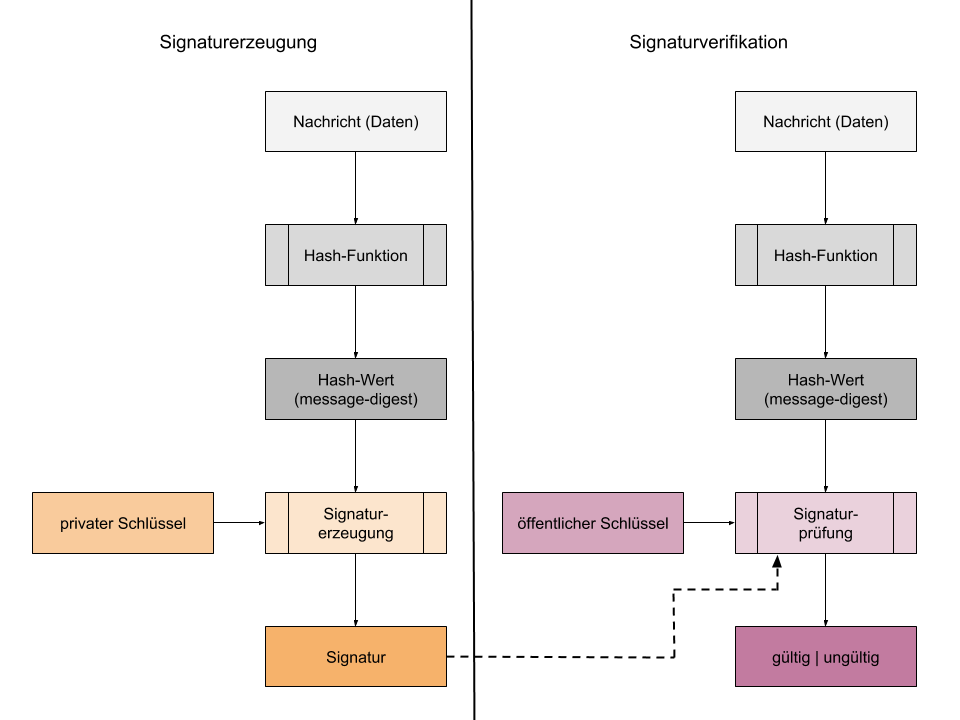
\includegraphics[width=\textwidth]{Abbildungen/Ablauf_Signatur.png}
    \caption{Schematischer Ablauf der Signaturerzeugung und Verifikation}
    \label{fig:Signaturablauf}
\end{figure}
Es gibt Grundsätzlich zwei Arten eine Nachricht $M$ digital zu signieren, wobei $S$ und $V$ zwei Personen sind \cite[S. 28-29]{kryptSec11}:
\begin{enumerate}
    \item Signatur mit Nachrichten-Rückgewinnung: Die Nachricht $M$ wird ohne Vorverarbeitung mit dem \textit{privaten Schlüssel} $d_s$ von $S$ signiert, sodass die daraus resultierende Signatur die Form $s = f_{d_s}(M)$ hat. Diese Nachricht kann von $V$ wiederrum durch den \textit{öffentlichen Schlüssel} $e_s$ von $S$ dechiffriert und die ursprüngliche Nachricht wiederhergestellt werden: $M = f_{e_s}(f_{d_s}(M))$. Nur geeignet für Nachrichten kürzer als die Schlüssellänge.
    \item Signatur mit Hashwert-Anhang: Die Nachricht $M$ wird mit Hilfe einer Hash-Funktion\footnote{Siehe Abschnitt \ref{sec:Hash-Funktionen}} $h(M)$ auf einen Wert mit konstanter Länge (z.B. 160 Bit) abgebildet. Die Signatur hat somit die Form $s = f_{d_s}(h(M))$ und wird zusätzlich zur Nachricht übertragen. Die Person $V$ kann nun den Hash-Wert der Nachricht $M$ durch $h(M) = f_{e_s}(f_{d_s}(h(M))$ errechnen. Auch geeignet für längere Nachrichten.
\end{enumerate}
In der Praxis findet nur die Signatur mit Hash-Wert Anhang Verwendung, da sonst die Signatur linear mit der Größe der Nachricht wächst. Welche Signaturalgorithmen $f_{d_s}(h(M))$ in der Praxis verwendet werden, wird hauptsächlich über das fortlaufend aktualisierte ``Digital Signature Standard (DSS)'' des National Institute of Standards and Technology in den USA vorgegeben. Dieses Dokument stellt Empfehlungen dar, welche Signaturalgorithmen als sicher angesehen werden können und wie diese zu verwenden sind. In Deutschland veröffentlicht das Bundesamt für Sicherheit in der Informationstechnik ebenfalls ein Dokument, welches solche Empfehlungen tätigt.

Auf Grundlage der Empfehlung des Bundesamt für Sicherheit in der Informationstechnik \cite[Kapitel 5.4]{bsi-tr-02102-1} möchte ich zur Übersicht die gängigen Signaturverfahren aufzählen:
\subsection{RSA}
Der \textbf{R}iverst-\textbf{S}hamir-\textbf{A}dleman Algorithmus ist ein Public-Key Kryptosystem und findet oft Anwendung in Bereichen der Verschlüsselungsverfahren. Jedoch kann dieser Algorithmus auch zur Signatur von Nachrichten eingesetzt werden. 
\begin{quote}
    ``Die Sicherheit von RSA basiert auf der Schwierigkeit, große Zahlen in ihre Primfaktoren zu zerlegen.'' \cite[S. 82]{ertel12}
\end{quote}
\subsubsection{Schlüsselerzeugung}
Zwei stochastisch undabhängige Primzahlen $p$ und $q$ werden generiert, wobei $p \neq q$. Die beiden Primzahlen sollten so groß gewählt werde, dass das RSA-Modul $n=p \cdot q$ die gewünschte Stellenlänge hat. Das Schlüsselpaar besteht aus $e$ (encrypt) und $d$ (decrypt) und wird mit Hilfe der Eulerschen Funktion ermittelt:
\[
    \Phi(n = p \cdot q) = (p-1) \cdot (q-1)
\]
Einer der Beiden Schlüssel wird zufallsmäßig gewählt, sodass er kleiner ist als $\Phi(n)$ und teilerfremd zu $\Phi(n)$ ist. Der andere Schlüssel ergibt sich aus der Bedingung für RSA, dass die beiden Schlüssel $e$ und $d$ eines Paares multiplikativ invers in der Arithmetik modulo $\Phi(n)$ sind:
\[
    e \cdot d \equiv \bmod \Phi(n) 
\]
Der \textit{private Schlüssel} $d$ ist geheim und muss durch spezielle Maßnahmen geschützt werden, da er für die Signatur benutzt wird. Der \textit{öffentliche Schlüssel} $e$ und der Modulo $n$ werden veröffentlicht und dienen zur Verifikation der Signatur. Die Primzahlen $p$ und $q$ müssen ebenfalls sicher verwahrt werden oder können vernichtet werden um Missbrauch vorzubeugen.
\subsubsection{Signaturerzeugung}
Vorraussetzung für die Signaturerzeugung, ist die Formatierung\footnote{RSA-Padding} des Hash-Wertes auf die Länge des Moduls $n$. Die Signatur $s$ für die Nachricht $M$ kann nun berechnet werden durch:
\[
    s = (M^d) \bmod n    
\]
\subsubsection{Signaturverifikation}
Die Signatur kann wiederrum unter Kenntnis des \textit{öffentlichen Schlüssels} bestehend aus $(e, n)$ verifiziert werden:
\[
    (s^e) \bmod n = (M^d)^e \bmod n = M'
\]
Falls die wiederhergestellte Nachricht $M'$ mit der übertragenen Nachricht $M$ übereinstimmt, so kann die Signatur als gültig angesehen werden.e
\subsubsection{Anmerkungen}
Bei RSA handelt es sich um ein deterministisches Verfahren. In der Praxis wird statt der unmittelbaren Nachricht, der Hash-Wert dieser Nachricht signiert. In diesem Fall muss $m$ mit $h(m)$ ersetzt werden. Besonders die Erzeugung der Zufallszahlen und der \textit{private Schlüssel} sind von besonderer Wichtigkeit und müssen durch spezielle Verfahren geschützt werden, auf die ich im Laufe der Arbeit \todo{Kapitel referenzieren} noch detailliert eingehen werde.

\subsection{Digital Signature Algorithm (DSA)}
Dieses Signaturverfahren wurde erstmals 1991 vom National Institute of Standards and Technology vorgeschlagen und letztendlich auch im Jahr 1994 als Standard im Digital Signature Standard (DSS) offiziell aufgenommen \cite[S. 125]{krypt08}.
\begin{quote}
    ``Die Sicherheit dieses Verfahrens beruht auf der [..] Schwierigkeit des Diskreten Logarithmenproblems $\mathbb{F}^*_p$.'' \cite[S. 45]{bsi-tr-02102-1}
\end{quote}
Dieses Verfahren ist speziell für den Anwendungsbereich der \textit{digitalen Signatur} eingeführt worden und eignet sich nicht, im Gegensatz zu RSA, zur kryptographischen Verschlüsselung von Nachrichten. Ein weiterer Unterschied zu RSA ist das Benötigen einer kryptographischen Hash-Funktion zur Signaturerzeugung.
\subsubsection{Schlüsselerzeugung}
Wähle zwei Zahlen:
\[
    (L, N) \in \{(1024, 160), (2028, 224), (2048, 256), (3072, 256)\}
\]
Anschließend werden die Primzahlen $p$ und $q$ mit folgenden Eigenschaften erzeugt:
\[
    2^{N-1} < q < 2^N \quad\textrm{,}\quad 2^{L-1} < p < 2^L \quad\textrm{und}\quad q|(p-1)
\]
Zusätzlich wird eine Zahl $\alpha \in \mathbb{F}^*_p$ gewählt und $g$ berechnet:
\[
    g := \alpha^{(p-1)/q} \bmod p
\]
Falls $g = 1$ wiederhole die Berechnung von $g$ mit einem anderen $\alpha \in \mathbb{F}^*_p$. Der letzte Schritt der Schlüsselerzeugung besteht aus der Wahl einer Zahl $x \in \{1, \ldots, q - 1 \}$ und $y := g^x \bmod p$. Der \textit{öffentliche Schlüssel} setzt sich zusammen aus $(p, q, g, y)$ und der \textit{private Schlüssel} aus $x$.

Wie auch bei RSA, wird der \textit{private Schlüssel} zur Signaturerzeugung genutzt und muss geschützt werden. Der \textit{öffentliche Schlüssel} dient wiederrum auch der Verifikation der Signatur.
\subsubsection{Signaturerzeugung}
Die Erzeugung der Signatur benötigt eine Hash-Funktion. Dabei sollte eine empfohlene Funktion aus der Tabelle \ref{table:Hashfunktionen} verwendet werden. Der aus der Funktion resultierende Hash-Wert sollte der Bit-Länge von $q$ entsprechen. Ebenso sollte die Länge von $p$ mindestens 2000 betragen\footnote{Bis 2022 als sicher eingestuft.}.

Zur Berechnung wird noch eine Zufallszahl $k \in \{ 1, \ldots, q - 1 \}$ benötigt. Diese Zahl wird pro Signatur erzeugt und muss, wie der \textit{private Schlüssel}, sicher verwaltet werden. Die Signatur einer Nachricht $M$ welche durch das DSA Verfahren generiert wird, besteht aus dem Zahlenpaar $r$ und $s$:
\[
    r = (g^k \bmod p)
\]
Zur Berechnung von $s$ muss ausserdem eine Zahl $z$ bestimmt werden aus den linkesten $N$ Bits des Hash-Wertes $h(M)$:
\[
    s = (z + xr)k^{-1} \bmod q
\]
Die Signatur, bestehend aus $(s, r)$ kann nun zusammen mit der Nachricht $M$ verifiziert werden.
\subsubsection{Signaturverifikation}
Um die Signatur, bestehend aus $(s, r)$, auf der Nachricht $M$ zu prüfen, bedarf es des \textit{öffentlichen Schlüssels} $(p, q, g, y)$ des Unterzeichners. Im ersten Schritt wird überprüft ob: 
\[
    0 < r < q \quad\textrm{und}\quad 0 < s < q
\]
Falls einer dieser beiden Bedingungen nicht erfüllt werden, ist die Signatur als ungültig anzusehen. Damit die Signatur als gültig angesehen werden kann, muss $v$ berechnet werden durch:
\begin{align*}
    v& = (((g)^{u1}(y)^{u2}) \bmod p) \bmod q \quad\textrm{, mit}\\
    w& = (s)^{-1} \bmod q \\
    z& = \textrm{linkeste N Bits von $h(M)$} \\
    u1& = (zw) \bmod q \\
    u2& = (rw) \bmod q
\end{align*}
Falls $v = r$, ist die Signatur gültig.
\subsubsection{Anmerkungen}
Im Gegensatz zur RSA-Signaturvariante handelt es sich hierbei um einen probabilistischen Algorithmus, da die zufällige Wahl des \textit{privaten Schlüssels} mit $x \in \{1, \ldots, q - 1 \}$ essenziell ist. Wichte schützenswerte Merkmale dieses Verfahrens sind der \textit{öffentliche Schlüssel} $x$ und die Zufallszahl $k$ aus der Signaturerzeugung.

\section{Mobile Signaturen}
Durch den Entwurf der EU-Richtlinie 1999/93/EG wurde die gesetzliche Grundlage für rechtsverbindliche elektronische Signaturen geschaffen. Die Richtlinie sieht eine Gerüst von Anforderungen für die Technologien rund um die elektronische Signaturen vor, basierend auf einer Zertifizierungstelle\footnote{Auch Certificate Authority oder CA genannt.}, welche die \textit{öffentlichen Schlüssel} zertifiziert und so genannten ``sicheren Signaturerstellungseinheiten'' (SSEE), welche wiederrum die \textit{privaten Schlüssel} des Benutzers verwaltet. Die EU-Kommission unterscheidet dabei zwischen der elektronischen Signatur und der \textit{qualifizierten} elektronischen Signatur (QES). Eine QES muss folgende Anforderungen erfüllen \cite{eSigEU99}:
\begin{enumerate}
    \item Sie ist eindeutig einem Unterzeichner zugeordnet.
    \item Sie ist in der Lage, den Unterzeichner zu identifizieren.
    \item Sie wird mit Mitteln erstellt, die der Unterzeichner unter seiner alleinigen Kontrolle hat.
    \item Sie ist mit den Daten, auf die sie sich bezieht, so verknüpft, dass jede spätere Änderung der Daten erkennbar ist.
\end{enumerate}
Die klassische Variante eines SSEE ist die Smartcard, welche mit einem Kartenlesegerät angeschlossen an einem Computer bedient wird und die privaten Schlüssel enthält sowie die mathematischen Operationen einer Signatur durchführen kann. Diese Variante verhindert jedoch die Mobilität des Anwenders und erfordert zusätzliche Hardware, was folglich zu einer schwachen Adaption im privaten Sektor geführt hat. Eine Alternative dazu bieten die \textit{mobilen Signaturen}, welche durch mobile Endgeräte, wie z.B. Mobiltelefone, umgesetzt werden. Nach Rossnagel \cite{rossnagel}, können \textit{mobile Signaturen}   in zwei Varianten klassifiziert werden:
\begin{itemize}
    \item \textbf{Serverseitige mobile Signaturen:} Bei der serverseitigen mobilen Signatur wird die Signatur auf einem (zentralen) Server erstellt. Dazu müssen die kryptographischen Schlüssel auf dem Server verwaltet werden. Der Benutzer muss durch besondere Authentifizierungsmethoden den Zugriff auf diese Schlüssel autorisieren.
    \item \textbf{Clientseitige mobile Signaturen:} Bei der clientseitigen mobilen Signatur wird die Signatur durch ein sicheres Signaturerstellungsgerät (z.B. Smartcard) auf dem Mobilgerät des Benutzers erstellt. Die kryptographischen Schlüssel liegen somit dem Benutzer selbst vor und müssen von diesem sicher verwaltet werden.
\end{itemize}

\section{Handy-Signatur}
Die \textit{Handy-Signatur} ist ein österreichisches (Fern-)Signaturverfahren und gehört der Gruppe der serverseitigen mobilen Signaturen an. Sie erlaubt es dem Benutzer sich eindeutig im Internet per Mobiltelefon zu authentifizieren. Die Signatur ist eine \textit{qualifizierte elektronische Signatur} und ist der handgeschriebenen Unterschrift per Gesetz\footnote{Nach EU-Richtlinie 1999/93/EG\cite{eSigEU99}} gleichgesetzt. Nach Angaben der A-Trust GmbH, welche für die Entwicklung und die technische Infrastruktur der \textit{Handy-Signatur} zuständig sind, sind aktuell ca. eine Millionen Nutzer registriert und es werden rund 18.000 Signaturen täglich ausgelöst \cite{atrustHSig}.
\begin{quote}
    ``Egal ob Steuererklärung, Gewerbeanmeldung, Kindergeldbeantragung, FinanzOnline- oder ELGA-Abfragen: Mit der Handy-Signatur können bereits mehrere 100 Formulare digital unterschrieben werden. Amtswege und andere Rechtsgeschäfte, die die eindeutige Personenidentifikation erfordern, sind so an 365 Tagen im Jahr, 24 Stunden am Tag, möglich. Die UserInnen sind nicht mehr an die begrenzten Öffnungszeiten von Ämtern, Banken und Unternehmen gebunden.

    Im Zuge der digitalen Transformation wird eine sichere Authentifizierung im Internet immer wichtiger, um eine verlässliche Identifikation von Personen und Organisationen ortsunabhängig und länderübergreifend zu ermöglichen.'' \cite{atrustHSig}
\end{quote}
Da es sich bei der \textit{Handy-Signatur} um eine Fern-Signatur handelt, hat der Benutzer dabei keinen direkten Zugriff auf das Schlüsselpaar, welches zur Erzeugung der Signatur nötig ist. Dieses wird stattdessen von der A-Trust GmbH verwaltet. Das Auslösen der qualifizierten elektronischen Signatur über das Online-Portal läuft wie folgt ab (Siehe Abb. \ref{fig:HandySignaturablauf} \cite[S. 3, Abb. 1]{mobQes}):
\begin{enumerate}
    \item Benutzer greift auf eine Web-basierte Schnittstelle eines Service Providers zu.
    \item Service Provider schickt standardisierte Signaturanfrage an A-Trust.
    \item Über eine Web-Schnittstelle des Service-Providers gibt der Benutzer seine Mobilfunknummer und sein Passwort ein und versendet sie über eine gesicherte HTTPS-Verbindung.
    \item Eine Transaktionsnummer (TAN) wird von A-Trust an den Mobilfunkanbieter des Benutzers gesendet.
    \item Die TAN wird vom Mobilfunkanbieter an den Benutzer weitergeleitet.
    \item Die TAN wird vom Benutzer über eine gesicherte Verbindung zu A-Trust übetragen.
    \item Signaturerstellung wird von A-Trust durchgeführt und Ergebnis an den Service Provider gemeldet.
    \item Service Provider meldet das Ergebnis an den Benutzer über die Web-Schnittstelle.
\end{enumerate}
\begin{figure}[htbp]
    \centering
        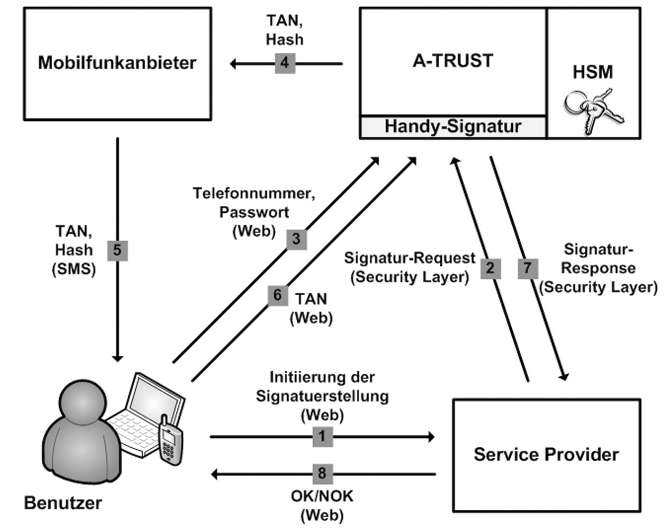
\includegraphics[width=\textwidth]{Abbildungen/Ablauf_Handy-Signatur.png}
    \caption{Schematischer Ablauf der Handy-Signatur}
    \label{fig:HandySignaturablauf}
\end{figure}
Dabei ist zu beachten, dass dieser Vorgang nicht vom gleichen Endgerät ausgeführt werden soll, welches die SMS erhalten hat, da sonst keine \textit{qualifizierte elektronische Signatur} erstellt werden kann. Das Sicherheitskonzept der Anwendung basiert auf der Kombination von üblicher Passwortauthentifizierung und der \textit{Out-Of-Band Authentifizierung} als zweiten Faktor. Der Zugriff auf den \textit{privaten Schlüssel} zur Signaturerstellung muss also, erstens durch ein Passwort und zweitens durch den separaten Kanal des Mobilfunknetzes, autorisiert werden. Die eigentliche Signaturerstellung wird von A-Trust in einem zentralem HSM\footnote{Hardware Sicherheits-Modul} vorgenommen, welches die kryptographischen Schlüssel des Benutzers sicher verwahrt.
\subsubsection{Vorteile}
Der Vorteil der Anwendung, gegenüber der Verwendung der Chipkarte (Bürgerkarte), ist die Verwendung des SMS-TAN als Authentifizierungsmethode, statt eines Kartenlesegerätes am Computer des Benutzers. Somit soll eine maximale Verfügbarkeit der Anwendung sichergestellt werden, da die SMS-TAN von beliebigen Mobiltelefonen mit SIM-Karte empfangen werden kann. Außerdem bietet die \textit{Out-Of-Band Authentifizierung} einen zusätzlichen Schutz, falls der Computer des Benutzers kompromittiert sein sollte.
\subsubsection{Nachteile}
Genau in der Tatsache, dass der Authentifizierungscode über eine SMS empfangen wird, liegt auch der größte Nachteil des Verfahrens. Während man eine Chipkarte gewohnheitsmäßig sicher verwahrt und der Zugriff darauf nur über spezielle Hardware mit einem PIN geschehen kann, ist das Mobiltelefon ein Alltagsgegenstand. Des weiteren ist nicht das Endgerät selbst für den Empfang des Authentifizierungscodes zuständig, sondern die Mobiltelefonnummer welche über die SIM-Karte beim Telekomunikationsdienstleister hinterlegt ist. Da die Mobiltelefonnummer kein sicheres Merkmal von Besitz ist, bekommt das Passwort welches zur Anmeldung im Online-Portal genutzt wird eine hohe Bedeutung. Wer Zugriff auf die Mobiltelefonnummer und das Zugangspasswort erlangt, hat die Möglichkeit im Namen dieser Person rechtskräftige Verträge abzuschließen\todo{Wikipedia zitieren?}. 

\section{Authentifizierung}
asdasd

% ----------------------------------------------------------------
% Quellcodeverzeichnis
% ----------------------------------------------------------------
\clearpage
\phantomsection
\addcontentsline{toc}{chapter}{Quellcodeverzeichnis}
\listoflistings
\clearpage

% ----------------------------------------------------------------
% Tabellenverzeichnis
% ----------------------------------------------------------------
\phantomsection
\addcontentsline{toc}{chapter}{Tabellenverzeichnis}
\listoftables
\clearpage

% ----------------------------------------------------------------
% Abbildungsverzeichnis
% ----------------------------------------------------------------
\phantomsection
\addcontentsline{toc}{chapter}{Abbildungsverzeichnis}
\listoffigures
\clearpage

% ----------------------------------------------------------------
% Literaturverzeichnis
% ----------------------------------------------------------------
\phantomsection
\addcontentsline{toc}{chapter}{Literaturverzeichnis}
\bibliographystyle{ieeetr}
\bibliography{Literaturverzeichnis}

\end{document}